\chapter{Oversigt over spørgeskemaspørgsmål}
\label{app:FlowdiagramSPG}
%
Spørgeskemaet blev brugt i forbindelse med undersøgelsen af hvilke semaforiske gestikker, der skal knyttes til de forskellige funktioner. Spørgeskemaet er dynamisk opbygget, så testpersonerne får ikke nødvendigvis de samme spørgsmål, da spørgsmålene i nogle tilfælde afhænger af tidligere svar. Spørgeskemaet blev udarbejdet i SurveyXact.\blankline
%
På \autoref{fig:FlowdiagramSpg} fremgår en oversigt over de spørgsmål testpersonerne responderer på, inden de præsenteres for videoerne. Testlederen angiver, hvilket nummer testpersonen er, før testpersonen selv besvarer spørgeskemaet. Køn angives ved at afkrydse enten: \textit{Kvinde}, \textit{Mand} eller \textit{Andet} og alder angives ved at indtaste talværdier. Efterfølgende angiver testpersonerne, ved afkrydsning, om de er højre- eller venstrehåndet. Herefter angiver testpersonerne, ved afkrydsning af \textit{Ja} eller \textit{Nej}, om de har brugt gestikker i nogle produkter, hvor de ikke skulle røre ved en skærm, dertil er der en forklarende tekst: \textit{Eksempelvis i spilkonsoller}. Afkrydses \textit{Nej} sendes testpersonen videre til spørgsmål, om de har et eller flere B$\&$O produkter, jævnfør \autoref{fig:FlowdiagramSpg}. Afkrydses \textit{Ja} skal testpersonerne angive, i hvilke produkter de har brugt gestikker, hvor de ikke skulle røre ved en skærm. Dette sker ligeledes ved afkrydsning af en eller flere muligheder: \textit{Xbox (Kinect)}, \textit{Nintendo Wii}, \textit{Leap Motion}, \textit{Smartphones}, \textit{Tablets}, \textit{Virtuel Reality briller} eller \textit{Andet}, i tilfælde af at testpersonerne afkrydser \textit{Andet} skal de angive produktet. Dernæst skal testpersonerne angive, hvor erfarne de vurderer, at de selv er med gestikker, hvilket gøres ved at afkrydse en af følgende muligheder: \textit{Meget erfaren}, \textit{Erfaren}, \textit{Uerfaren} eller \textit{Meget uerfaren}. 

Når testpersonerne har angivet dette ender de ved spørgsmålet \textit{Har du et eller flere B$\&$O produkter?}, jævnfør \autoref{fig:FlowdiagramSpg}. Spørgsmålet stilles som et \textit{Ja}/\textit{Nej} spørgsmål, hvor testpersonerne, hvis de afkrydser \textit{Ja}, efterfølgende bliver bedt om at angive, hvilke B$\&$O produkter de har. Afkrydses \textit{Nej} derimod vidersendes de til spørgsmålet \textit{Jeg betragter mig selv som}, hvor testpersonerne, der afkrydsede \textit{Ja} ligeledes sendes til, efter de har angivet hvilket B$\&$O produkt de har. Dette spørgsmål besvares ved at afkrydse én af følgende muligheder: \textit{Værende den første til at anskaffe mig den nyeste teknologi}, \textit{Værende lige så hurtig, som andre til at anskaffe mig den nyeste teknologi} eller \textit{Værende den sidste til at anskaffe mig den nyeste teknologi}. Når dette spørgsmål er besvaret, er testpersonerne færdig med de indledende spørgsmål, jævnfør \autoref{fig:FlowdiagramSpg}.
%
\begin{figure}[H]
	\centering
	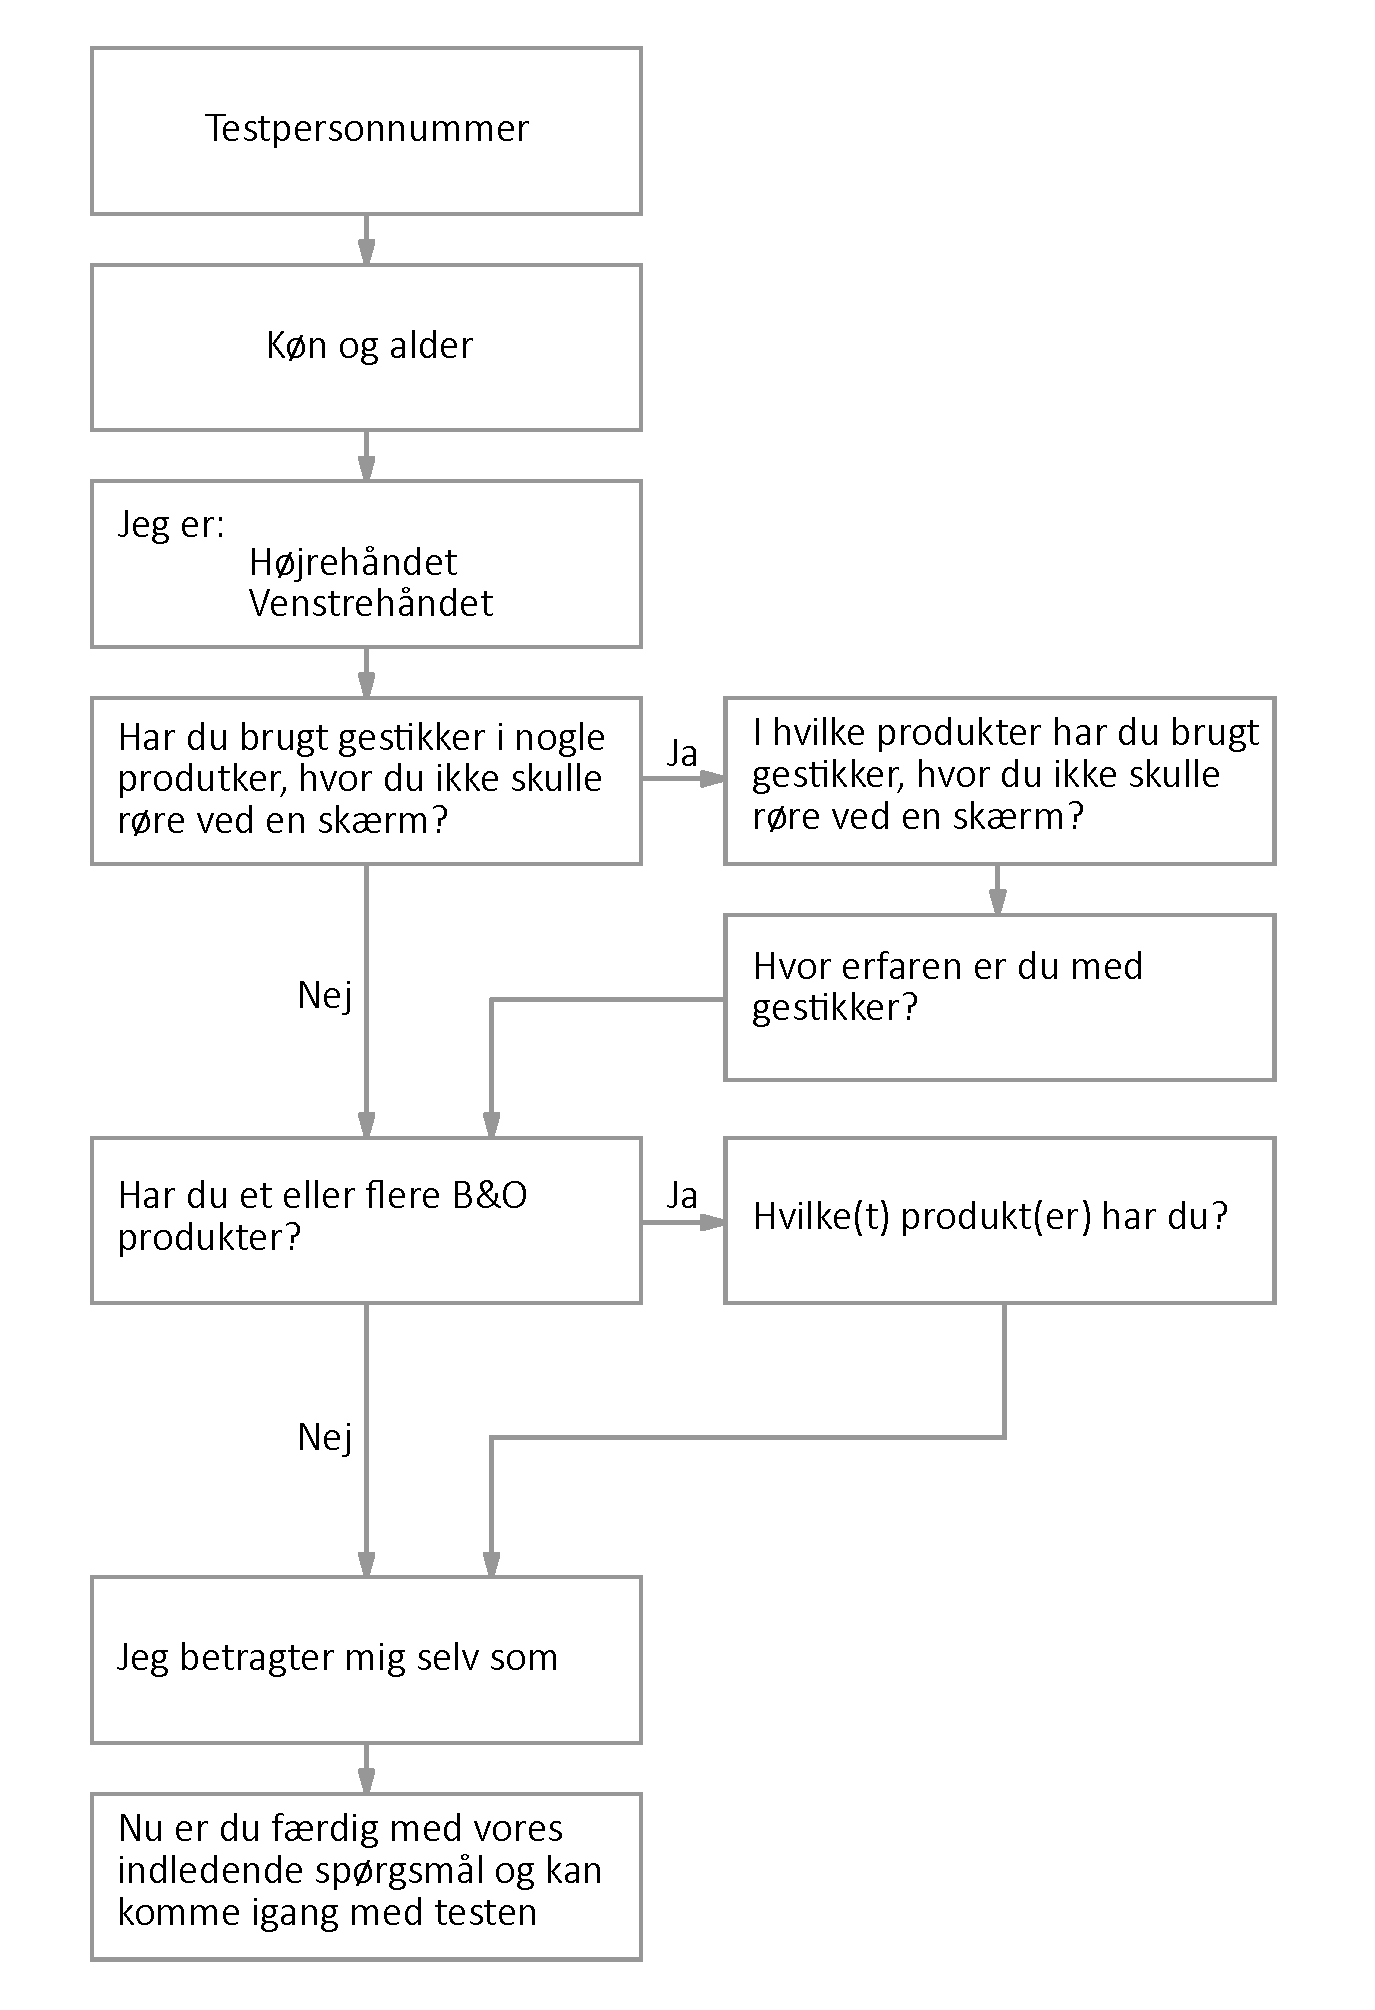
\includegraphics[resolution=300,width=0.9\textwidth]{Test1/FlowdiagramSpg}
	\caption{Oversigt over spørgsmål i spørgeskemaet, uden svarmulighederne.}
	\label{fig:FlowdiagramSpg}
\end{figure}
\noindent
%